\documentclass[a4paper,12pt]{article}
\usepackage{amsmath,amssymb,amsfonts,amsthm}
\usepackage{tikz}
\usepackage [utf8x] {inputenc}
\usepackage [T2A] {fontenc} 
\usepackage[russian]{babel}
\usepackage{cmap} 
\usepackage{ gensymb }
% Так ссылки в PDF будут активны
\usepackage[unicode]{hyperref}
\usepackage{ textcomp }
\usepackage{indentfirst}
\usepackage[version=3]{mhchem}

% вы сможете вставлять картинки командой \includegraphics[width=0.7\textwidth]{ИМЯ ФАЙЛА}
% получается подключать, как минимум, файлы .pdf, .jpg, .png.
\usepackage{graphicx}
% Если вы хотите явно указать поля:
\usepackage[margin=1in]{geometry}
% Или если вы хотите задать поля менее явно (чем больше DIV, тем больше места под текст):
% \usepackage[DIV=10]{typearea}

\usepackage{fancyhdr}

\newcommand{\bbR}{\mathbb R}%теперь вместо длинной команды \mathbb R (множество вещественных чисел) можно писать короткую запись \bbR. Вместо \bbR вы можете вписать любую строчку букв, которая начинается с '\'.
\newcommand{\eps}{\varepsilon}
\newcommand{\bbN}{\mathbb N}
\newcommand{\dif}{\mathrm{d}}

\newtheorem{Def}{Определение}


\pagestyle{fancy}
\makeatletter % сделать "@" "буквой", а не "спецсимволом" - можно использовать "служебные" команды, содержащие @ в названии
\fancyhead[L]{\footnotesize Лабораторные работы по общей физике}%Это будет написано вверху страницы слева
\fancyhead[R]{\footnotesize ФУПМ МФТИ}
%\fancyfoot[L]{\footnotesize \@author}%имя автора будет написано внизу страницы слева
\fancyfoot[R]{\thepage}%номер страницы —- внизу справа
\fancyfoot[C]{}%по центру внизу страницы пусто

\renewcommand{\maketitle}{%
	\noindent{\bfseries\scshape\large\@title\ \mdseries\upshape}\par
	\noindent {\large\itshape\@author}
	\vskip 2ex}
\makeatother
\def\dd#1#2{\frac{\partial#1}{\partial#2}}


\title{1.2. Эффект Комптона}
\author{Хурсик Екатерина} 

\begin{document}
	
\maketitle
\section*{Цель работы}

1)С помощью сцинтиляционного спектрометра исследовать энергетический спектр $\gamma$-квантов,
рассеянных на графите. 2)Определить энергию рассеянных $\gamma$-квантов в зависимости
от угла рассеяния, 3)а также энергию покоя частиц, на которых происходит комптоновское рассеяние.

\section{Метод достижения цели}

\subsection*{2)}

Для определения энергии $\gamma$-квантов нужно исследовать кривую распределения по амплитуде 
электрических импульсов на выходе ФЭУ (Под действием монохроматического излучения на выходе ФЭУ возникает
распределение электрических импульсов. В памяти компьютера происходит накопление числа
пришедших импульсов в соответствии с их амплитудой и при помощи специальной программы компьютер
выводит на экран гистограмму, по оси иксов которого откладывается амплитуда анализирующего импульса
(она же номер канала), а по оси игреков -- число импульсов заданной амплитуды в данном канале.)

Устанавливая сцинтиляционный счётчик под разными углами $\theta$ к первоначальному
направлению полёта $\gamma$-квантов и вводя значения этих углов в ЭВМ, снимаем амплитудные
спектры и определим положения фотопиков для каждого значения угла $\theta$.

\subsection*{3)}

Для определения энергии покоя частиц, на которых происходит комптоновское рассеяние:
\begin{itemize}
	\item Строим график, откладывая по оси иксов $1-\cos\theta$, а по оси игреков $\frac{1}{N(\theta)}$. Проводим через полученные точки наилучшую прямую.
	\item Пользуемся графиком и формулой $E_r = E_{\gamma}=\frac{N_\text{наил}(90)}{N_\text{наил}(0)-N_\text{наил}(90)}$. (Пересечение построенной прямой с осью игреков определяет значение $N_\text{наил}(0)$, а пересечение этой прямой с прямой $\cos\theta=0$ даёт значение $N_\text{наил}(90)$.)
\end{itemize}


	
\section{Ход работы}
Устанавливая сцинтиляционный счётчик под разными углами $\theta$ к первоначальному
направлению полёта $\gamma$-квантов и вводя значения этих углов в ЭВМ, снимим амплитудные
спектры и определим положения фотопиков для каждого значения угла $\theta$.

Измерения будем проводить с шагом $10^\circ$ в диапазоне от $0^\circ$ до $120^\circ$.

Результаты измерений:
\begin{figure}[h!]
    \begin{center}
		\centering
		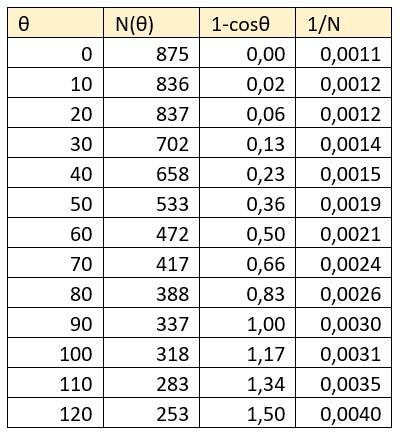
\includegraphics[width=0.5\linewidth]{2020-10-22.jpg}
    \end{center}
\end{figure}

\pagebreak
Построим график $\frac{1}{N}(1-\cos\theta)$:
\begin{figure}[h!]
    \begin{center}
		\centering
		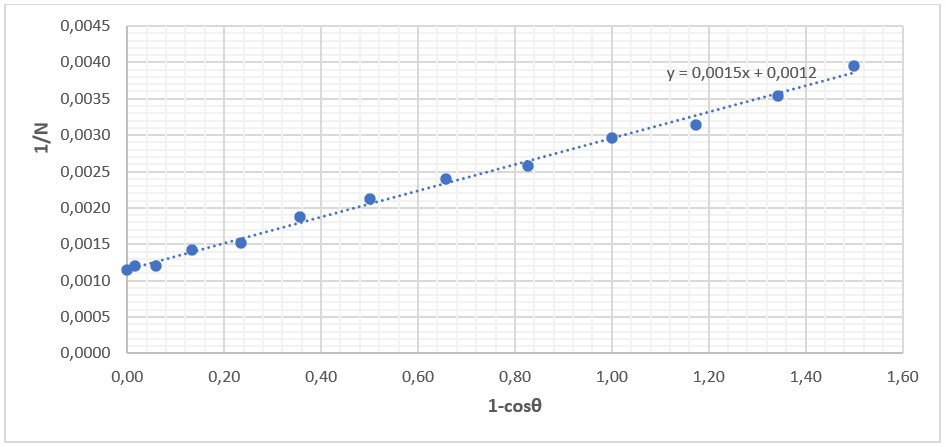
\includegraphics[width=1.1\linewidth]{2020-10-15.jpg}
    \end{center}
\end{figure}

По данным графика рассчитаем энергию покоя электронов:

при $\theta=0^\circ$: $\quad\frac{1}{N}=k(1-\cos\theta)+b\quad\rightarrow\quad\frac{1}{N}=b+k$\\

при $\theta=90^\circ$: $\quad\frac{1}{N}=k(1-\cos\theta)+b\quad\rightarrow\quad\frac{1}{N}=b$\\
\begin{equation}
	E_r = E_{\gamma}=\frac{N_\text{наил}(90)}{N_\text{наил}(0)-N_\text{наил}(90)} = \frac{\frac{1}{(b+k)}}{\frac{1}{b}-\frac{1}{(b+k)}}=\frac{b}{k}=527 \, \text{МэВ}
\end{equation}

$\varepsilon=3,8\%\quad\rightarrow\quad E_r=(527\pm20) \, \text{МэВ}$
\section{Выводы}

1) Достаточно точно определили энергию рассеянных $\gamma$-квантов в зависимости
от угла рассеяния. Для этого в формулу $E_r= E_{\gamma}=\frac{N(90)}{N(0)-N(90)}$
подставили значения $N_\text{наил}(0)$ и $N_\text{наил}(90)$, полученные с помощью
графика. Это позволило уменьшить роль случайных погрешностей, вызванных, например,
колебаниями напряжения, существенно влияющими на ФЭУ.

2) Определили энергии покоя частиц, на которых происходит комптоновское рассеяние,
которая в пределах погрешности совпадает с табличной.
					
\end{document}

